\section{Documentazione API}
In questa sezione vengono mostrate alcune delle API sviluppate per l’iterazione 2. 
È possibile visualizzare tutte le API mediante la collezione di Postman presente nella repository GitHub.
Tra tutte le APIs sviluppate, le piu significative offrono le seguenti funzionalità.
\begin{itemize}
    \item API per la creazione di un evento.
    \item API per la creazione di una prenotazione.
    \item API per la visualizzazione di prenotazioni di uno specifico utente.
    \item API per la registrazione di un profilo.
\end{itemize}


\newpage

\begin{figure}[h!]
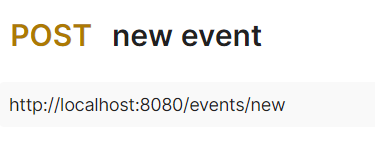
\includegraphics[width=7cm]{test/postman/tnewevent.PNG}\\
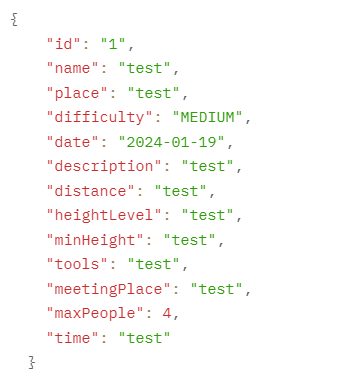
\includegraphics[width=7cm]{test/postman/newevent.PNG}\\
\caption{Creazione nuovo evento}
\end{figure}

\begin{figure}[h!]
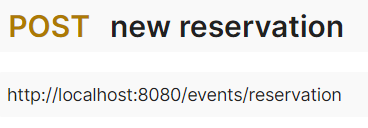
\includegraphics[width=7cm]{test/postman/tnewres.PNG}\\
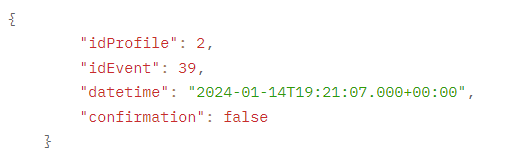
\includegraphics[width=7cm]{test/postman/newres.PNG}\\
\caption{Inserimento nuova prenotazione}
\end{figure}

\begin{figure}[h!]
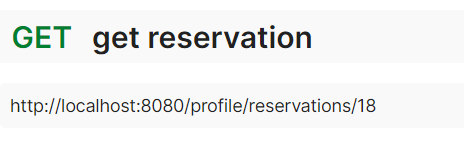
\includegraphics[width=7cm]{test/postman/getreservation.PNG}\\
\caption{Prenotazione dato uno specifico profilo}
\end{figure}

\begin{figure}[h!]
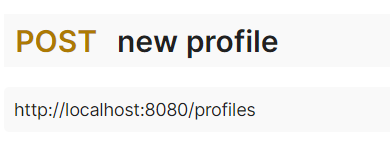
\includegraphics[width=7cm]{test/postman/tnewprofile.PNG}\\
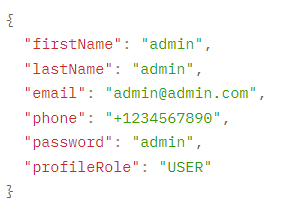
\includegraphics[width=7cm]{test/postman/newprofile.PNG}\\
\caption{Creazione nuovo profilo}
\end{figure}
